% In Z[i], b = 3+i is a side divisor of the blue points and an exact
% divisor of the red points: rounding x+iy to the nearest multiple r·(3+i)
% lands within distance 1.
% Source: book/tex/H113/ring-flavors.tex (§ When is a ring a Euclidean domain?).
\documentclass[border=2mm]{standalone}
\usepackage{tikz}
\begin{document}
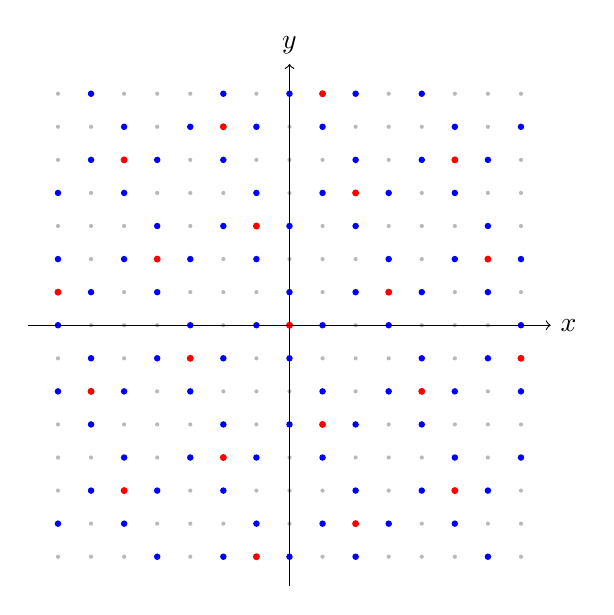
\begin{tikzpicture}[scale=0.42]
  \foreach \x in {-7,...,7}{
    \foreach \y in {-7,...,7}{
      \pgfmathtruncatemacro{\rre}{round((3*\x+\y)/10)}
      \pgfmathtruncatemacro{\rim}{round((3*\y-\x)/10)}
      \pgfmathsetmacro{\bx}{3*\rre-\rim}
      \pgfmathsetmacro{\by}{\rre+3*\rim}
      \pgfmathsetmacro{\dist}{veclen(\x-\bx,\y-\by)}
      \pgfmathtruncatemacro{\cls}{(\dist<0.01)?2:((\dist<1.01)?1:0)}
      \ifcase\cls
        \fill[gray!55] (\x,\y) circle (1.8pt);
      \or
        \fill[blue] (\x,\y) circle (2.8pt);
      \or
        \fill[red] (\x,\y) circle (3pt);
      \fi
    }
  }
  \draw[->] (-7.9,0) -- (7.9,0) node[right] {$x$};
  \draw[->] (0,-7.9) -- (0,7.9) node[above] {$y$};
\end{tikzpicture}
\end{document}
